\documentclass[10, letterpaper]{article}
\usepackage[utf8]{inputenc}
\usepackage[english]{babel}
 
\newtheorem{definition}{Definition}\usepackage{bussproofs}
\usepackage{mathtools}
\usepackage{nopageno}
\usepackage{graphicx}
\usepackage{graphicx,caption}
\usepackage{dsfont}
\usepackage{subcaption}
\usepackage[]{algorithm2e}
\usepackage{scalerel}
\usepackage[usenames, dvipsnames]{color}

\begin{document}

\subsection*{Introduction} 
\paragraph{}
Our contracts are consisted of three different parts: two {\bf super nodes}, one {\bf clause}, and a {\bf red vis edge}. \\ 
The interpretation for the red vis edge is that  \emph{"the vis relation that must be enforced"}. We call the two special effects connected by this edge $\eta_s$ and $\eta_d$. \\
Super nodes (depicted as blue circles in the figures) have two different types: StartNode, which contains the beginning of the red vis edge starts and EndNode where the vis edge ends. \\
\begin {figure} [h]
\centering
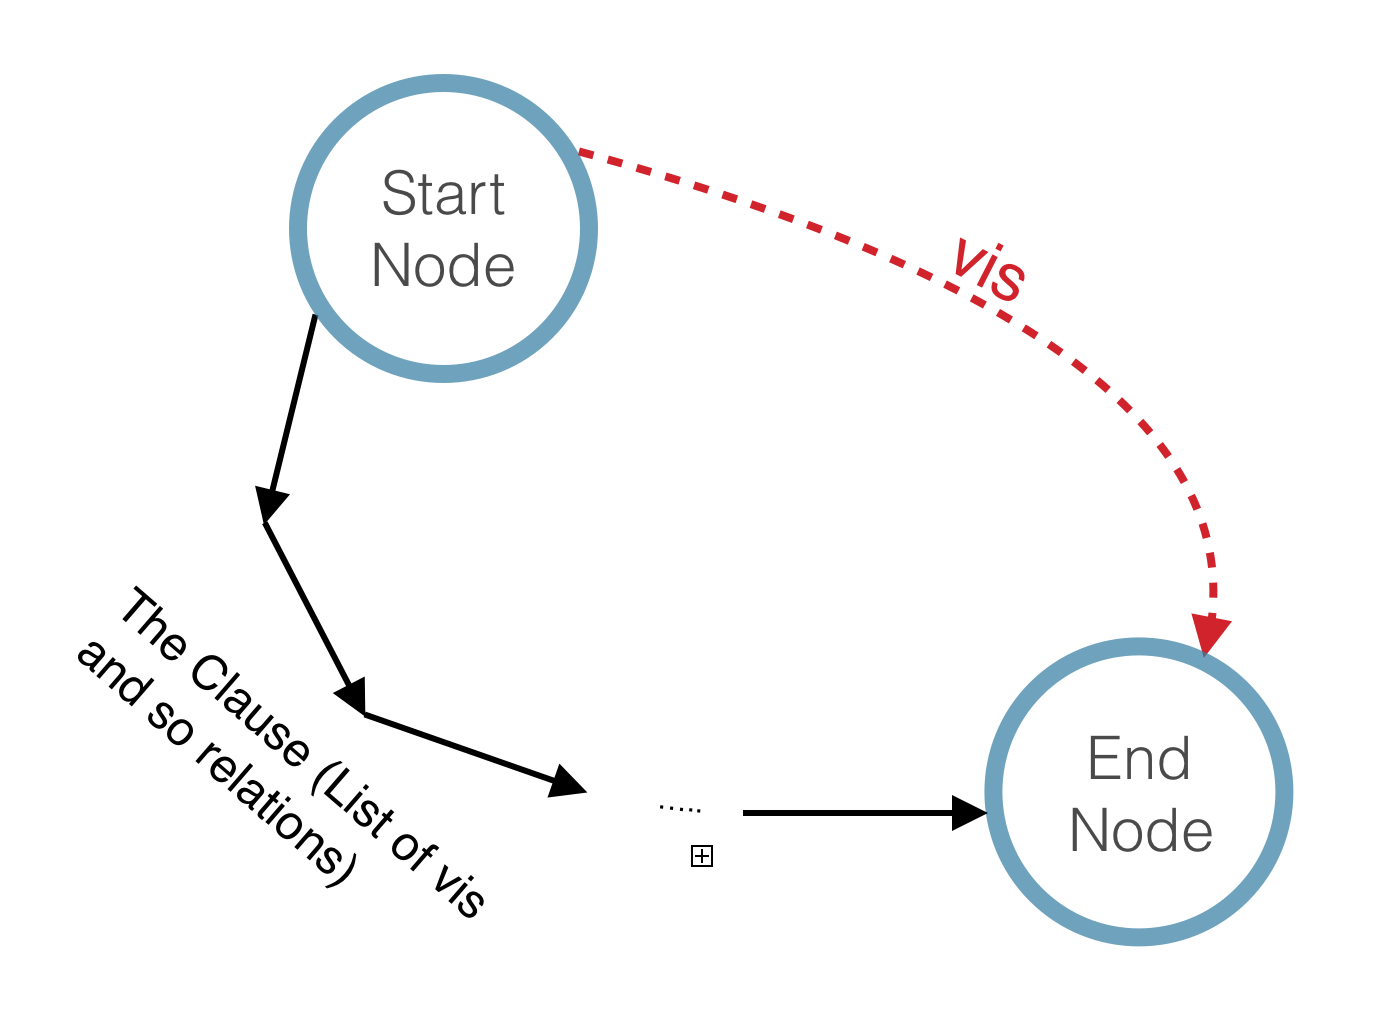
\includegraphics [scale=0.25] {general.png} 
\caption {General form of a contract (The blue circles can contain either a single effect, or two effect connected by a $txn$ edge) }
\end {figure}


Super Nodes are just syntactical packages for different types of consistency requirements: for session guarantees (without transactions) the super nodes are just $\eta_s$ or $\eta_d$. However, to capture  the transactional requirements it can include two effects that are related by $txn$ relation, which relates the operations from a transaction in their session order. 

\begin {figure} [h]
\centering
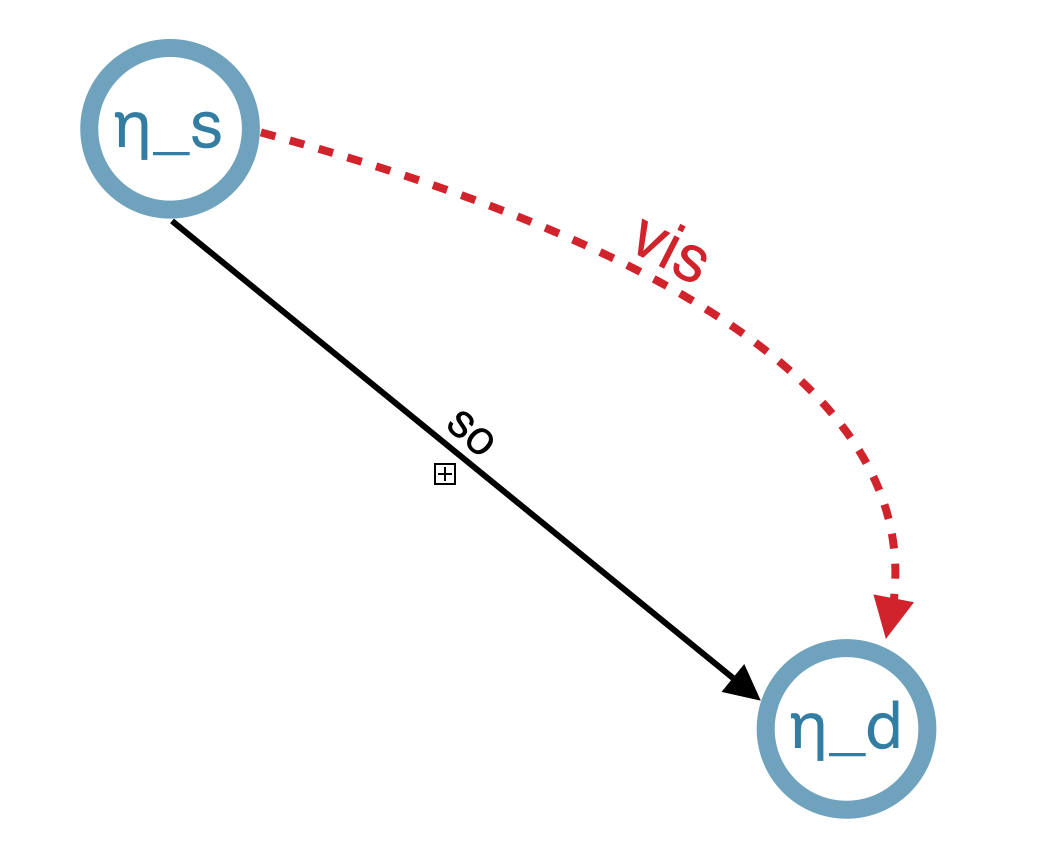
\includegraphics [scale=0.25] {rmw} 
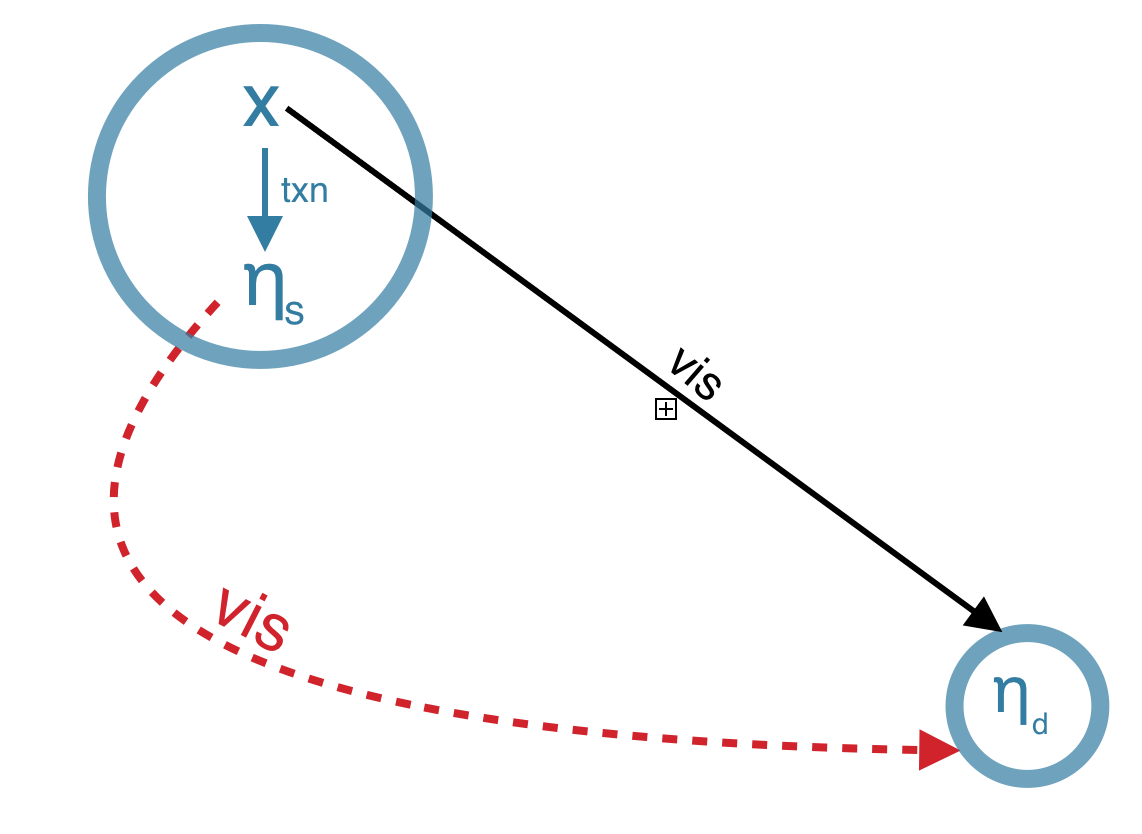
\includegraphics [scale=0.25] {rc} 

\caption {Two examples: left is RMW with no transaction and single effects at super nodes. The right figure however captures RC with its StartNode containing $x \xrightarrow{txn} \eta_s$}
\end {figure}

I believe the system is complete for all contracts of this type, and the language is also able to generate the known interesting contracts. 



\subsection*{Syntax}
\begin{figure}[h]
	\centering
	\begin{minipage}{.75\textwidth}
		$\eta_s,\eta_d, x \in$ EffVis   \hspace {25 mm}  $Op \in $ OperationName \\
		$N_s \in $ StartNode   ::=    $\eta_s | x \xrightarrow{txn} \eta_s | \eta_s \xrightarrow{txn} x$ \\
		$N_e \in $ EndNode ::= $\eta_d | x \xrightarrow{txn} \eta_d $ \\
		$R \in $ Relation ::= $vis | so | R \cup R $ \\ 
		$C \in $ Clause ::= $[R] | R^*$ \\		
		$\pi \in$ Prop ::= $(<N_s,N_e>,C) | \pi \vee \pi$ \\
		%$\tau \in $ EffectType ::= $Op | \tau \vee \tau$ \\
		$\psi \in$ Contract ::= $ \pi \Rightarrow {\color{Red} vis (\eta_s,\eta_d)}$ 
		\caption{The Contract Language}
		\label{fig:ctrt}
	\end{minipage}
\end{figure}
\vspace{10 mm}
\subsection*{Examples}



\begin {itemize}
	\item {\bf Read My Write (RMW)}
	\subitem $ (<\eta_s,\eta_d> , [so])  \Rightarrow {\color{Red} vis (\eta_s,\eta_d) } $
	\item {\bf Monotonic Reads (MR)}
	\subitem $ (<\eta_s,\eta_d> , [vis,so] )  \Rightarrow {\color{Red}vis (\eta_s,\eta_d) }$
	\item {\bf Monotonic Writes (MW)}
	\subitem $ (<\eta_s,\eta_d> , [so,vis] )   \Rightarrow {\color{Red} vis (\eta_s,\eta_d)} $
	\item {\bf Writes Follow Reads (WFR)}
	\subitem $[(<\eta_s,\eta_d> , [vis,vis]) \vee (<\eta_s,\eta_d> , [vis,so,vis])] \Rightarrow {\color{Red} vis (\eta_s,\eta_d)}  $
	\item {\bf Read Committed (RC)}
	\subitem $ (<x \xrightarrow{txn} \eta_s,\eta_d> , [vis])  \Rightarrow {\color{Red}vis (\eta_s,\eta_d) } $
	\item {\bf Monotonic Atomic View (MAV)}
	\subitem $ (<\eta_s,x \xrightarrow{txn} \eta_d > , [vis])  \Rightarrow {\color{Red} vis (\eta_s,\eta_d)} $
	

\end {itemize}











\end{document}